\documentclass[tikz]{standalone}% 'crop' is the default for v1.0, before it was 'preview'
\usepackage{pgfplots}

\definecolor{tucol1}{rgb}{1.0 0.5 0.05}
\definecolor{tucol2}{rgb}{0.52,0.72,0.10}
\definecolor{tucol3}{rgb}{0.0 0.0 0.8}
\definecolor{tucol5}{rgb}{0.8 0.8 0}
\definecolor{tucol4}{rgb}{0.8 0 0.8}
\definecolor{tucol6}{rgb}{0 0.8 0.8}

\begin{document}
	\tikzset{
  annotated cuboid/.pic={
    \tikzset{%
      every edge quotes/.append style={midway, auto},
      /cuboid/.cd,
      #1
    }
    \draw [every edge/.append style={pic actions, densely dashed, opacity=.5}, pic actions]
    (0,0,0) coordinate (o) -- ++(-\cubescale*\cubex,0,0) coordinate (a) -- ++(0,-\cubescale*\cubey,0) coordinate (b) edge coordinate [pos=1] (g) ++(0,0,-\cubescale*\cubez)  -- ++(\cubescale*\cubex,0,0) coordinate (c) -- cycle
    (o) -- ++(0,0,-\cubescale*\cubez) coordinate (d) -- ++(0,-\cubescale*\cubey,0) coordinate (e) edge (g) -- (c) -- cycle
    (o) -- (a) -- ++(0,0,-\cubescale*\cubez) coordinate (f) edge (g) -- (d) -- cycle;
    %\node at (b)+(0,-5pt) {\filters};
    %\path [every edge/.append style={pic actions, |-|}]
    %(b) +(0,-5pt) coordinate (b1) edge [""'] (b1 -| c);
    %(b) +(-5pt,0) coordinate (b2) edge ["\cubey \cubeunits"] (b2 |- a)
    %(c) +(3.5pt,-3.5pt) coordinate (c2) edge ["\cubez \cubeunits"'] ([xshift=3.5pt,yshift=-3.5pt]e)
    %;
  },
  /cuboid/.search also={/tikz},
  /cuboid/.cd,
  width/.store in=\cubex,
  height/.store in=\cubey,
  depth/.store in=\cubez,
  units/.store in=\cubeunits,
  scale/.store in=\cubescale,
  filters/.store in = \filters
  width=10,
  height=10,
  depth=10,
  units=cm,
  scale=.1,
  filters={},
}

\begin{tikzpicture}[shorten >=1pt,-,draw=black!50]]
    \tikzstyle{every pin edge}=[->,shorten <=1pt]
    \tikzstyle{layer}=[rectangle, minimum height=80pt, minimum width=1pt, inner xsep=0]
    \tikzstyle{conv}=[layer,fill=blue]
    \tikzstyle{pool}=[layer, fill=green]
    \tikzstyle{spp}=[layer, fill=red]
    \tikzstyle{fc}=[layer, fill=black]
    \tikzstyle{cube}=[opacity=.5,very thick,fill=red]
    \tikzstyle{legend}=[rectangle, draw=black, minimum width=1em, minimum height=1em, text width=1em, inner xsep=0]
	
	%include the input image
	%\node[rotate=45] at (-0.8,-0.1) {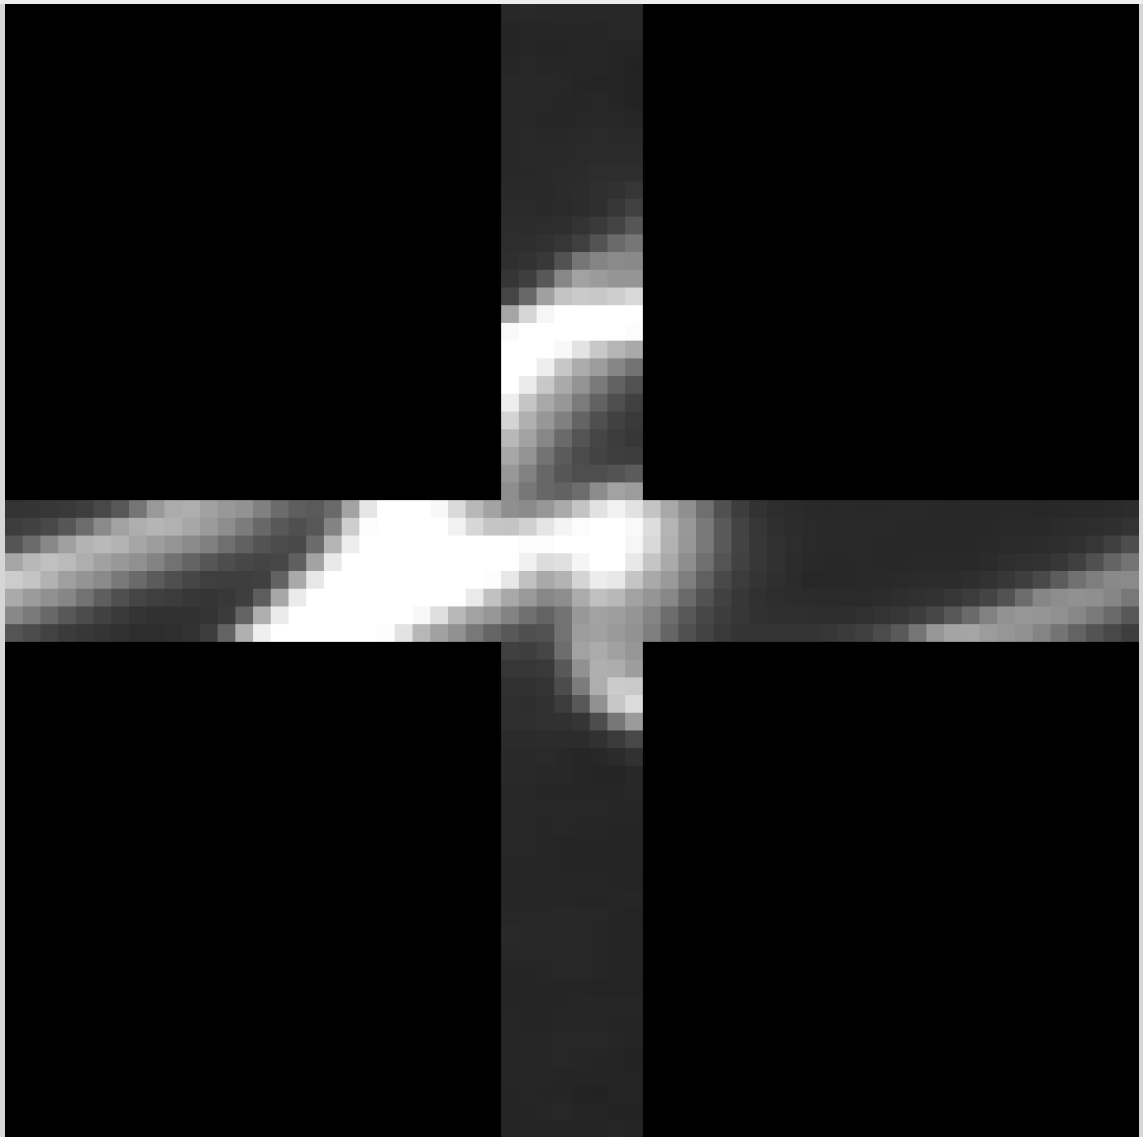
\includegraphics[width=2cm]{lrc_sample_inside.png}};
	
	% conv part
	\pic [fill=tucol2!50, draw=tucol2] at (0,0.4) {annotated cuboid={width=1, height=40, depth=80}};
	\pic [fill=tucol2!50, draw=tucol2] at (1.0,0.4) {annotated cuboid={width=1, height=40, depth=80}};
	
	\pic [fill=tucol1!50, draw=tucol1] at (2,0) {annotated cuboid={width=1, height=30, depth=60}};
	
	\pic [fill=tucol2!50, draw=tucol2] at (3,0) {annotated cuboid={width=2, height=30, depth=60}};
	%\pic [fill=tucol2!50, draw=tucol2] at (2.2,0) {annotated cuboid={width=2, height=20, depth=40}};
	
	\pic [fill=tucol1!50, draw=tucol1] at (4,0) {annotated cuboid={width=1, height=20, depth=40}};
	
	\pic [fill=tucol2!50, draw=tucol2] at (5,0) {annotated cuboid={width=4, height=20, depth=40}};
	
	\pic [fill=tucol1!50, draw=tucol1] at (6,0) {annotated cuboid={width=1, height=10, depth=20}};
	
	\pic [fill=tucol2!50, draw=tucol2] at (7,0) {annotated cuboid={width=4, height=10, depth=20}};
	\pic [fill=tucol2!50, draw=tucol2] at (8,0) {annotated cuboid={width=4, height=10, depth=20}};
	
	
%	\pic [fill=tucol2!50, draw=tucol2] at (4.4,0) {annotated cuboid={width=4, height=10, depth=20}};
%	\pic [fill=tucol2!50, draw=tucol2] at (5.2,0) {annotated cuboid={width=4, height=10, depth=20}};
%	\pic [fill=tucol2!50, draw=tucol2] at (6.0,0) {annotated cuboid={width=4, height=10, depth=20}};
%	\pic [fill=tucol2!50, draw=tucol2] at (6.8,0) {annotated cuboid={width=4, height=10, depth=20}};
%	\pic [fill=tucol2!50, draw=tucol2] at (7.6,0) {annotated cuboid={width=4, height=10, depth=20}};
%	\pic [fill=tucol2!50, draw=tucol2] at (8.8,0) {annotated cuboid={width=8, height=10, depth=20}};
%	\pic [fill=tucol2!50, draw=tucol2] at (10.0,0) {annotated cuboid={width=8, height=10, depth=20}};
%	\pic [fill=tucol2!50, draw=tucol2] at (11.2,0) {annotated cuboid={width=8, height=10, depth=20}};
%	\pic [fill=tucol2!50, draw=tucol2] at (13.2,0) {annotated cuboid={width=16, height=10, depth=20}};
%	\pic [fill=tucol3!50, draw=tucol3] at (14.4,0) {annotated cuboid={width=8, height=10, depth=20}};
	
	 MLP part
	%\pic [fill=red!50, draw=red] at (10.5,-2) {annotated cuboid={width=2, height=2, depth=80}};
	\pic [fill=black!50, draw=black] at (8.5,-1.4) {annotated cuboid={width=2, height=2, depth=60}};
	\pic [fill=black!50, draw=black] at (9.5,-1.4) {annotated cuboid={width=2, height=2, depth=60}};
	%\pic [fill=magenta!50, draw=magenta] at (12.7,-1.5) {annotated cuboid={width=2, height=2, depth=40}};
	\pic [fill=cyan!50, draw=cyan] at (12.5,0.5) {annotated cuboid={width=2, height=2, depth=10}};
	\pic [fill=cyan!50, draw=cyan] at (11.5,-0.4) {annotated cuboid={width=2, height=2, depth=10}};
	\pic [fill=cyan!50, draw=cyan] at (10.5,-1.4) {annotated cuboid={width=2, height=2, depth=10}};
	
	% plot the filter numbers
	\node[rotate=45] at (-0.1, -3.9) {\footnotesize{32}};
	\node[rotate=45] at (0.9, -3.9) {\footnotesize{32}};
	
	%\node[rotate=45] at (0.8, -3.3) {\footnotesize{128}};
	\node[rotate=45] at (2.9, -3.3) {\footnotesize{64}};
	
	\node[rotate=45] at (4.8, -2.3) {\footnotesize{128}};
	
	\node[rotate=45] at (6.8, -1.3) {\footnotesize{256}};
	\node[rotate=45] at (7.8, -1.3) {\footnotesize{256}};
%	\node[rotate=45] at (5.78, -1.3) {\footnotesize{256}};
%	\node[rotate=45] at (6.58, -1.3) {\footnotesize{256}};
%	\node[rotate=45] at (7.38, -1.3) {\footnotesize{256}};
%	\node[rotate=45] at (8.4, -1.3) {\footnotesize{512}};
%	\node[rotate=45] at (9.55, -1.3) {\footnotesize{512}};
%	\node[rotate=45] at (10.7, -1.3) {\footnotesize{512}};
	
	\node[rotate=45] at (8.3, -1.9) {\footnotesize{256}};
	\node[rotate=45] at (9.3, -1.9) {\footnotesize{256}};
	\node at (13.3, 0.5) {\footnotesize{inside}};
	\node at (12.6, -0.4) {\footnotesize{intersects}};
	\node at (11.5, -1.3) {\footnotesize{outside}};
	
	% plot the legend
	\node[legend, fill=tucol2!50, label=right:{$3\times3$ Convolutional Layer + ReLU}] at (-0.5, -5) {};
	\node[legend, fill=tucol1!50, label=right:{$2\times2$ Max Pooling Layer}] at (-0.5, -5.5) {};
	%\node[legend, fill=red!50, label=right:{$3$-level Spatial Pyramid Max Pooling Layer}] at (0, -6) {};
	\node[legend, fill=black!50, label=right:{Fully Connected Layer + ReLU}] at (6.5, -5) {};
	%\node[legend, fill=magenta!50, label=right:{Fully Connected Layer + Linear Activation}] at (7, -5.5) {};
	\node[legend, fill=cyan!50, label=right:{Local Region Classification}] at (6.5, -5.5) {};
\end{tikzpicture}

\end{document} 
